\chapter{Probabilidade}

\section*{Objetivo: Definir um modelo estatístico que seja adequado à descrição e interpretação de fenômenos aleatórios.}
\subsection{Conceitos básicos}
\begin{description}

  \item [Experimentos ou fenômenos aleatórios ($\varepsilon$)]: são os acontecimentos cujos resultados não podem ser previstos 
    com certeza, sob condições idênticas.

    \begin{description}
      \item [Exemplos]:

        \begin{itemize}
          \item Lançamento de um dado.
          \item Lançamento de uma moeda.
          \item Tempo de vida útil de um componente eletrônico.
        \end{itemize}
    \end{description}
  \item [Espaço Amostral ($\Omega$):] refere-se ao conjunto de todos os possíveis resultados de um experimento ou fenômeno 
    aleatório.
    \begin{description}
      \item [Exemplos]:
        \begin{enumerate}[label=$\Omega_{\arabic*}$]
          \item $= \{ 1,2,3,5,6 \}$ 
          \item $= \{ c,k \}$ Sendo $k$ cara, $c$ coroa.
        \item $= [ 0,\infty \}$ 
      \end{enumerate}
  \end{description}
\item [Evento:] qualquer subconjunto do espaço amostral $\Omega$ do experimento aleatório $\varepsilon$.
  \begin{description}
    \item[Notação: $A,B,C,D,\dots,A_1,A_2,A_3,\dots,B_1,B_2,\dots$]

    \item Notamos que, como $A$ é um evento então $A \subset \Omega$.

  \end{description}

\end{description}
\subsection{Tipos de Eventos}

\begin{description}
  \item [Evento Simples ou Elementar:] é o evento formado por um único ponto do espaço amostral. 
    \begin{description}
      \item [Exemplo:]
        $A=\{w \}$.
    \end{description}

  \item [Evento Composto:]  é o evento formado por dois ou mais pontos do espaço amostral.

    \begin{description}
      \item[Exemplo:]
        $ A= \{w_1,w_2,w_3 \}$
    \end{description}

  \item [Evento Certo:] é o evento formado por todos os pontos amostrais.
    \begin{description}
      \item    [Exemplo]: $A= \Omega$ 
    \end{description}
  \item [Evento Impossível]: É o evento que não possuí elementos de $\Omega$, isto é, evento vazio.
    \begin{description}
      \item [Notação]: $A=\{\}$ ou $A= \emptyset$

      \item    [Alguns Exemplos]:
        \begin{itemize}[label=]
          \item  $A=$ Face do dado maior que 5.

            $A=\{6\}$

          \item    $B=$ Face do dado ser par.

            $B= \{2,4,6\}$

          \item    $C=$ Face do dado maior ou igual a 1.

            $C= \{1,2,3,4,5,6\}=\Omega$

          \item        $D=$ Face do dado maior que 6.


            $D=\{ \}$ ou $D=\emptyset$
        \end{itemize}


    \end{description}
\end{description}
%Aula 2 9/03/2017
\subsection{Operação com Eventos}
Para ilustrar graficamente eventos é costume utilizar-se dos mesmos diagramas de Venn utilizados na teoria de conjuntos.

Considere eventos definidos em um espaço amostral $\Omega$ de um experimento aleatório $\varepsilon$.

\begin{description}
  \item [União de eventos ($A \cup B$)]: é o evento formado por todos os elementos que pertencem a $A$, ou  $B$, ou ambos.
    \begin{figure}[H]
      \centering
      \input{tikz/Probabilidade/figura1.tikz}
      \caption{}
      \label{fig:1}
    \end{figure} 
  \item [Intersecção de eventos ($A \cap B$)]: é o evento formado pelos elementos que pertencem a $A$ e a $B$.
    \begin{figure}[H]
      \centering
      \input{tikz/Probabilidade/figura2.tikz}
      \caption{}
      \label{fig:2}
    \end{figure} 
    \begin{description}
      \item[Casos Particulares]:
        \begin{enumerate}
          \item Se $B \subset A$, então $A \cap B= B$ 

            \begin{figure}[H]
              \centering
              \def\firstcircle{(0,0) circle (1.0cm)}
\def\thirdcircle{(0:0) circle (1.8 cm)}

% Now we can draw the sets:
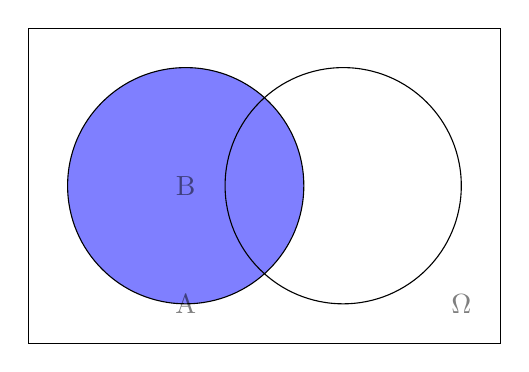
\begin{tikzpicture}
\begin{scope}[shift={(3cm,-5cm)}, fill opacity=0.5]
\draw (-2,-2) rectangle(4,2) ;
\node at (3.5,-1.5) {$\Omega$};
\fill[blue] \firstcircle;
\draw \firstcircle ;
\draw \thirdcircle ;
\node at (0,0) {B};
\node at (0,-1.5) {A};
\end{scope}
\end{tikzpicture}

              \caption{}
              \label{fig:3}
            \end{figure}

          \item Se $A$ e $B$ são eventos disjuntos ou mutuamente exclusivos (não possui elementos comuns), então $A\cap B = \emptyset$.

            \begin{figure}[H]
              \centering
              \def\firstcircle{(-0.5,0) circle (1.2cm)}
\def\thirdcircle{(0:2.5cm) circle (1.2cm)}

% Now we can draw the sets:
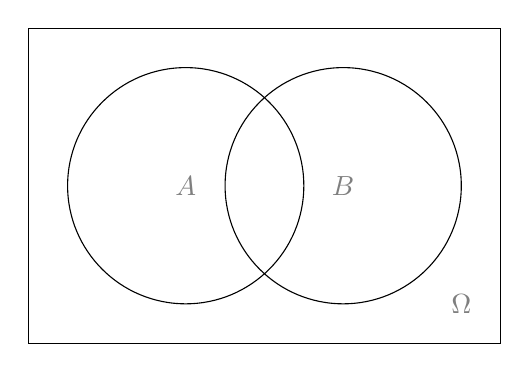
\begin{tikzpicture}
    \begin{scope}[shift={(3cm,-5cm)}, fill opacity=0.5]
\draw (-2,-2) rectangle(4,2) ;
\node at (3.5,-1.5) {$\Omega$};
        \draw \firstcircle node {$A$};
        \draw \thirdcircle node {$B$};
    \end{scope}
\end{tikzpicture}

              \caption{}
              \label{fig:4}
            \end{figure}

        \end{enumerate}
    \end{description}
  \item[Diferença de eventos ($A-B$)]: é o evento formado pelos elementos que pertencem a $A$ mas não pertencem a $B$.

    \begin{figure}[H]
      \centering
      \def\firstcircle{(0,0) circle (1.5cm)}
\def\thirdcircle{(0:2cm) circle (1.5cm)}

% Now we can draw the sets:
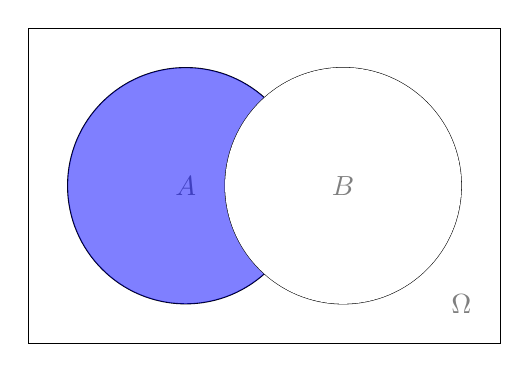
\begin{tikzpicture}
\begin{scope}[shift={(3cm,-5cm)}, fill opacity=0.5]
\draw (-2,-2) rectangle(4,2) ;
\node at (3.5,-1.5) {$\Omega$};

\draw \firstcircle node {$A$};
\fill[blue] \firstcircle;
\draw \thirdcircle ;
\fill[white,opacity=1] \thirdcircle;
\node at (2,0) {$B$};
\end{scope}
\end{tikzpicture}

      \caption{}
      \label{fig:5}
    \end{figure}
  \item [Evento Complementar ($\bar{A}$ ou $A^c$)]: é o evento formado por todos os elementos de $\Omega$ que não pertencem a $A$.
    \begin{description}
      \begin{figure}[H]
        \centering
        \def\firstcircle{(1,0) circle (1.5cm)}
\def \amostralspace{(-2,-2) rectangle (4,2)}
% Now we can draw the sets:
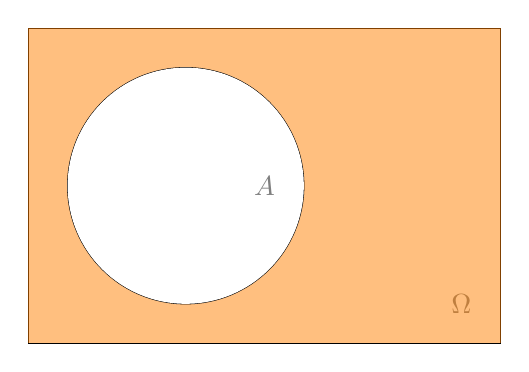
\begin{tikzpicture}
\begin{scope}[shift={(3cm,-5cm)}, fill opacity=0.5]
\draw \amostralspace ;
\node at (3.5,-1.5) {$\Omega$};

\fill[orange] \amostralspace;
\draw \firstcircle;
\fill[white,opacity=1] \firstcircle;
\clip \amostralspace;
\node at (1,0) {$A$};
\end{scope}
\end{tikzpicture}

        \caption{}
        \label{fig:6}
      \end{figure}

    \item [Alguns exemplos de eventos complementares]: 

      \begin{enumerate}[align=left,label=({\alph*}) ]

        \item $(A \cup B )^c = A^c \cap B^c$
          \begin{figure}[H]
            \centering
            \input{tikz/Probabilidade/figura7.tikz}
            \caption{}
            \label{figa:7}
          \end{figure}

        \item $(A \cap B)^c = A^c \cup B^c $
          \begin{figure}[H]
            \centering
            \input{tikz/Probabilidade/figura8.tikz}
            \caption{}
            \label{figura:8}
          \end{figure}

          Os itens ($a$) e ($b$) são conhecidos como Lei de Demorgan.
        \item $A \cup B^c = ( A \cap B ) \cup B^c = A \cup (A \cup B)^c$
          \begin{figure}[H]
            \centering
            \def\firstcircle{(0,0) circle (1.5cm)}
\def\thirdcircle{(2,0) circle (1.5cm)}

\def \amostralspace{(-2,-2) rectangle (4,2)}
% Now we can draw the sets:
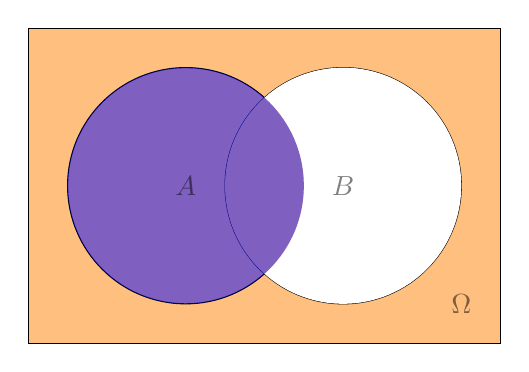
\begin{tikzpicture}
\begin{scope}[shift={(3cm,-5cm)}, fill opacity=0.5]
\draw[fill=orange] \amostralspace ;
\node at (3.5,-1.5) {$\Omega$};
\draw \thirdcircle;
\draw \firstcircle;
\fill[white,opacity=1] \thirdcircle;
\begin{scope}
\clip \thirdcircle;
\fill[orange] \firstcircle;
\end{scope}
\fill[blue] \firstcircle;
\node at (0,0){$A$};
\node at (2,0) {$B$};
\end{scope}
\end{tikzpicture}

            \caption{}
            \label{figura:9}

          \end{figure}

        \item  $A \cap B^c = B^c \cap (A \cup B)$
          \begin{figure}[H]
            \centering
            \def\firstcircle{(0,0) circle (1.5cm)}
\def\thirdcircle{(2,0) circle (1.5cm)}

\def \amostralspace{(-2,-2) rectangle (4,2)}
% Now we can draw the sets:
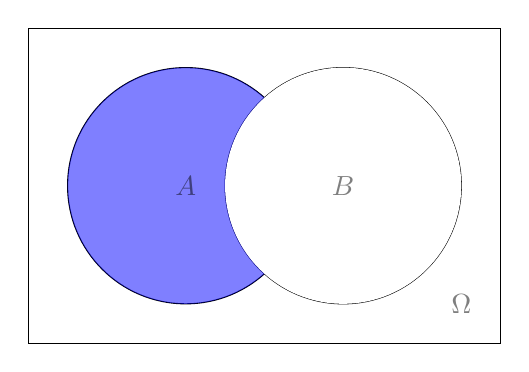
\begin{tikzpicture}
\begin{scope}[shift={(3cm,-5cm)}, fill opacity=0.5]
\draw \amostralspace ;
\node at (3.5,-1.5) {$\Omega$};
\draw \firstcircle;
\draw \thirdcircle;
\fill[blue] \firstcircle;
\fill[white,opacity=1] \thirdcircle;
\node at (0,0){$A$};
\node at (2,0) {$B$};
\end{scope}
\end{tikzpicture}

            \caption{}
            \label{fig:10}
          \end{figure}

      \end{enumerate}

    \item [Outras operações]: 

      \begin{enumerate}[leftmargin=*, label=\Roman*., widest=IV, align=left]
        \item     $A \cap \emptyset= \emptyset$ 
        \item     $A \cup \emptyset = A$ 
        \item     $\emptyset^{c} = \Omega$ 
        \item     $ \Omega^c = \emptyset$ 
        \item     $(A^c)^c = A$ 
        \item     $B= (A \cap B)\cup (A^c \cap B)$
        \item     $A= (A \cap B) \cup (A \cap B^c)$
      \end{enumerate}
    \item [Exemplo]: Escrever $A \cup B$ como união de eventos disjuntos.

      \begin{figure}[H]
        \centering
        \input{tikz/Probabilidade/figura1.tikz}
        \caption{}
        \label{fig:11}
      \end{figure}
      \begin{description}
        \item [Situação 1:]

          $(A \cup B) = A \cup (A^c \cap B)$

        \item      [Situação 2:]


          $A \cup B = B \cup (A \cap B^{c})$
      \end{description}

      Considerando a Situação 1 , vamos verificar se os eventos são disjuntos. Os eventos serão disjuntos se $A \cap ( A^c \cap B )= \emptyset$ . Vericando, temos: 
      \begin{align*}
        (A \cap A^c) \cap B = \emptyset \\
        \emptyset \cap B= \emptyset
      \end{align*}

  \end{description}
\end{description}
\section{Definições de Probabilidade}
\subsection{Probabilidade em Espaços Equiprováveis}
Se um experimento aleatório tiver $n$ resultados possíveis, $\Omega = \{ \omega_1,\omega_2,\ldots,\omega_n \}$, mutuamente exclusivos e igualmente possíveis e se um evento $A$ tiver $n_A$ desses resultados, então a probabilidade do evento $A$, representado por $P(A)$, é dada por: 
\begin{align}
  P(A)= \frac{N_a}{n}, \quad A \subset \Omega 
\end{align}
Sendo que $\Omega$ é definido como todo o espaco amostral, $n_A$ o número de casos favoráveis $A$ e $n$ o número de casos possíveis.

\begin{description}
  \item [Exemplo:] 

    Dado o lançamento de duas moedas honestas, calcule a probabilidade de: 
    \begin{enumerate}[label=(\alph*)]
      \item  Obter duas faces iguais.
      \item Obter pelo menos uma face diferente de cara
      \item  Obter pelo menos uma face diferente.
    \end{enumerate}
    \begin{figure} [H]
      \centering
      \begin{tabular}{c c c}
        \toprule
        &c&k\\ \cmidrule{2-3}
        c&(c,c)&(c,k)\\ \cmidrule{2-3}
        k&(k,c)&(k,k)\\    \bottomrule
      \end{tabular}
      \label{tab:1}
    \end{figure}
    \begin{align*}    \Omega = \{ (c,c); (c,k) ; (k,c) ; (k,k)\}
    \end{align*}
    \begin{enumerate}[label=(\alph*)]
      \item $A=$ Faces iguais
        \begin{align*}
          A= \{ (c,c) ; (k,k) \} \\
          P(A) = \frac{2}{4} = \frac{1}{2}= 0.5
        \end{align*}
      \item $B=$ Pelo menos uma face diferente de cara.

        \begin{align*}
          B= \{ (c,k) ; (k,c) ; (k,k) \} \\
          P(B)= \frac{3}{4}
        \end{align*}

      \item $C=$ Obter pelo menos uma face diferente

        \begin{align*}
          C= \{ (c,k) ; (k,c) \} \\
          P(C)= \frac{2}{4}= \frac{1}{2}
        \end{align*}
    \end{enumerate}

\end{description}
\subsection{Probabilidade Frequentista}

Um experimento é realizado  $n$ vezes, sendo $n$ um número grande. O evento $A$ ocorre exatamente $N_a$ vezes com: $0 \le N_a \le n$. A frequência relativa de vezes que ocorreu o evento $A$ é uma forma de aproximar a probabilidade do evento A, ou seja:
\begin{align}
  f_r (A)= \frac{n_a}{n} 
\end{align}
Quando $n \to \infty$, $f_r(A)$ aproxima-se de $P(A)$.
\begin{description}
  \item[Exemplo]: 

    Geração de $n$ número inteiros entre 1 e 5, $\{ 1,2,3,4,5 \}$, e o evento de interesse é a ocorrência do número 4.
\end{description}
\subsection{Probabilidade axiomática}

A probabilidade de um evento $A$ é definida como sendo um número $P(A)$ que satisfaz
os seguintes axiomas:
% Usar sempre numeração romana pra axiomas!
\begin{enumerate}[leftmargin=*, label=\Roman*., widest=IV, align=left]
  \item $P(A) > 0, \forall A \subset \Omega$ 
  \item $P(\Omega)=1$
  \item Se $A_1, A_2,\ldots$ são eventos mutuamente exclusivos ($A_i \cap A_j = \emptyset, \forall i \neq j$), então:
    \begin{align}
      P(\cup^\infty_{i=1} A_i)= P(A_1\cup A_2 \cup \ldots)= \sum \limits^\infty_{i=1} P(A_i) 
    \end{align}
\end{enumerate}
\begin{description}
  %14/03/2017
  \item[Propriedades]:

    \begin{enumerate}[label=(\alph*)]
      \item $0 \le P(A) \le 1$
      \item $P(\emptyset)=0$
      \item Se $A \subset \Omega$ então $P(A)=1-P(A^c)$
      \item Se $A \subset B \subset \Omega$, então $P(A) \le P(B)$
      \item Se $A,B \subset \Omega$, então vale:
        \begin{align}
          P(B)= P(B\cap A)+ P(B\cup \bar{A})
        \end{align}
      \item Se $A,B \subset \omega$, então:
        \begin{align}
          P(A\cup B)= P(A)+P(B)-P(A\cap B)
        \end{align}
      \item Se $A,B,C \subset \omega$, então:
        \begin{align}
          P(A\cup B \cup C)= P(A)+P(B)+P(C)-P(A \cap B)- P(A \cap C) \nonumber\\-
          P(B\cap C)+P(A\cap B \cap C) 
        \end{align}
    \end{enumerate}
  \item [Exemplo:] Mostre a propriedade $(g)$.

    Use o fato de que $A\cap (B \cup C )= (A\cap B )\cup (A \cap C )$:
    \begin{align*}
      P\left(A\cup B\cup C \right)\\
      = P\left(A \cup \left(B \cup C\right) \right)\\
      =P(A)+P(B\cup C)- P\left(A\cap \left(B\cup C \right) \right)\\
      =P(A)+P(B)+P(C)-P(B\cap C)- P\left((A \cap B)\cup (A \cap C)\right)\\
      =P(A)+P(B)+P(C)-P(B\cap C)\\
      - \left( P \left(A \cap B \right)+ P\left(A \cap C \right)-P\left(\left(A \cap B \right) \cap \left(A \cap C \right) \right) \right) \\
      =P(A)+P(B)+P(C)-P(B\cap C)- P(A \cap B)- P(A \cap C)+ P(A \cap B \cap C)
    \end{align*}

  \item [Exercício:]  Considere um experimento aleátorio e os eventos $A$ e $B$ associados, tais que:
    \begin{align*}
      P(A)= \frac{1}{2}\\
      P(B)= \frac{1}{3}\\
      P(A \cap B)= \frac{1}{4}
    \end{align*}
    Calcule as probabilidades:
    \begin{enumerate}[label=(\alph*)]
      \item $ P(\bar{A} \cap \bar{B})$
      \item $P(\bar{A} \cup \bar{B})$
    \end{enumerate}
    \begin{enumerate}[label=(\alph*)]
      \item \begin{align*}
          P(A^c \cap B^c) = 1- P(A \cup B) \\
          = 1- \{ P(A) + P(B) - P(A \cap B) \} \\
          =1 - \{ \frac{1}{2} + \frac{1}{3} -\frac{1}{4}\}= \frac{5}{12}
        \end{align*}
      \item \begin{align*}
          P(A^c \cup B^c) = P\left( \left( A \cap B\right)^c \right)\\
          = 1- P(A \cap B) = 1 - \frac{1}{4}= \frac{3}{4}
        \end{align*}  
        Ou de maneira similar:
        \begin{align*}
          P(A^c \cup B^c) = P(A^c) + P(B^c ) - P(A^c \cap B^c) \\
          = (1- P(A)) + (1- P(B)) - \frac{5}{12} \\
          = (1 - \frac{1}{2})+ (1 - \frac{1}{3})- \frac{5}{12}
        \end{align*}

    \end{enumerate}
    \subsection{Probabilidade Condicional}
    \begin{description}
      \item Sejam $A$ e $B$ dois eventos definidos em um mesmo espaco amostral $\Omega$.
        A probabilidade de $A$  dado que ocorre o evento $B$, denotada por $P(A/B)$ é definida por:
        \begin{align}
          P(A/B)= \frac{P(A\cap B)}{P(B)},  \quad P(B)>0. 
        \end{align}
        \begin{figure}[htpb]
          \centering
          \caption{Name}
          \label{fig:16}
        \end{figure}
        Consequentemente, podemos escrever:
        \begin{align}
          P(A\cap B)= P(A/B).P(B)
        \end{align}
        Conhecida como regra do produto.
      \item [Observação:]
        \begin{align}
          P(B/A)= \frac{P(B \cap A)}{P(A)}= \frac{P\left(A\cap B \right)}{P(A)}\\
          P(A \cap B)= P(B/A)\times P(A)
        \end{align}
        Logo:
        \begin{align}
          P(A \cap B) = P(B/A)\times P(A) \\
          =P(A/B)\times P(B)
        \end{align}
      \item [Exemplo]: Suponha que um escritório possua 100 computadores de tipos Desktop (D) e 
        Laptop (L) sendo alguns novos (N) e outro com um certo tempo de uso (U), distribuídos da seguinte forma:
        \begin{figure}[H] 
          \centering
          \begin{tabular}{c c c c}
            \toprule
            &D&L&Total\\ \cmidrule{2-4}
            N&40&30&70\\ \cmidrule{2-4}
            U&20&10&30\\ \cmidrule{2-4}
            Total&60&40&100 \\\bottomrule
          \end{tabular}
          \label{tab:2}
        \end{figure}

        Um funcionário escolhe um laptop ao acaso. Qual a probabilidade de que seja novo?

      \item[Resolução:]


        \begin{align*}
          P(N/L)= \frac{P(N \cap L)}{P(L)}= \frac{\frac{30}{100}}{\frac{40}{100}}=\frac{3}{4}
        \end{align*}

        Obs: $P(A \cap B)$ e $P(A/B)$
    \end{description}
    \section{Arvore de Probabilidades}

    Sejam $A,B \subset \Omega$. Uma representação bastante útil é a àrvore de probabilidades.
    \begin{description}
      \begin{figure}[H]
        \centering
        


% Set the overall layout of the tree
\tikzstyle{level 1}=[level distance=3.5cm, sibling distance=3.5cm]
\tikzstyle{level 2}=[level distance=3.5cm, sibling distance=2cm]

% Define styles for bags and leafs
\tikzstyle{bag} = [text width=4em, text centered]
\tikzstyle{end} = [circle, minimum width=3pt,fill, inner sep=0pt]

% The sloped option gives rotated edge labels. Personally
% I find sloped labels a bit difficult to read. Remove the sloped options
% to get horizontal labels. 
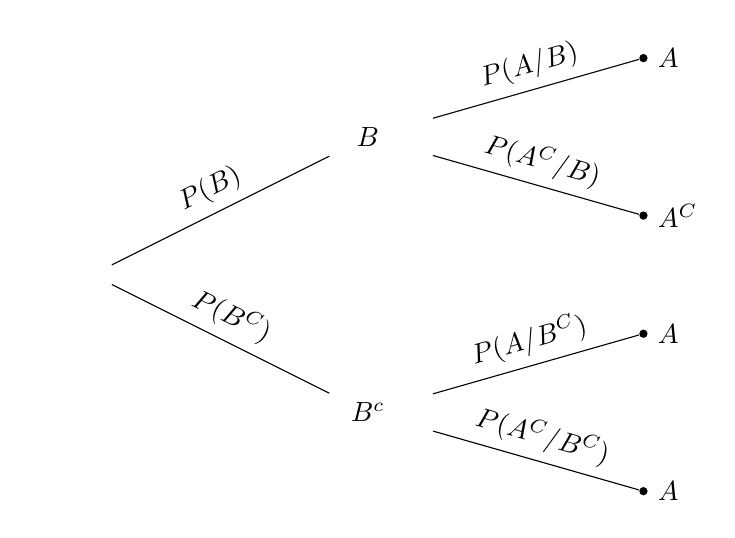
\begin{tikzpicture}[grow=right, sloped]
\node[bag] {}
    child {
      node[bag] {$B^{c}$}        
            child {
                node[end, label=right:
                    {$A$}] {}
                edge from parent
                node[above] {$P(A^{C}/B^C)$}
%                node[below]  {$\frac{4}{9}$}
            }
            child {
                node[end, label=right:
                    {$A$}] {}
                edge from parent
                node[above] {$P(A/B^C)$}
%                node[below]  {$\frac{5}{9}$}
            }
            edge from parent 
            node[above] {$P(B^{C})$}
%            node[below]  {$\frac{4}{7}$}
    }
    child {
        node[bag] {$B$}        
        child {
                node[end, label=right:
                {$A^{C}$}] {}
                edge from parent
                node[above] {$P(A^C/B)$}
%                node[below]  {$\frac{3}{9}$}
            }
            child {
                node[end, label=right:
                    {$A$}] {}
                edge from parent
                node[above] {$P(A/B)$}
%                node[below]  {$\frac{6}{9}$}
            }
        edge from parent         
        node[above] {$P(B)$}
%            node[below]  {$\frac{3}{7}$}
    };
  \end{tikzpicture}

        \label{fig:17}
        \caption{Um exemplo de uma àrvore de probabilidades}
      \end{figure}

    \item[Exemplo]: No exemplo anterior, qual a probabilidade de um funcionário selecionar um 
      desktop usado?
      \begin{figure}[H]
        \centering
        % Set the overall layout of the tree
\tikzstyle{level 1}=[level distance=3.5cm, sibling distance=3.5cm]
\tikzstyle{level 2}=[level distance=3.5cm, sibling distance=2cm]

% Define styles for bags and leafs
\tikzstyle{bag} = [text width=4em, text centered]
\tikzstyle{end} = [circle, minimum width=3pt,fill, inner sep=0pt]

% The sloped option gives rotated edge labels. Personally
% I find sloped labels a bit difficult to read. Remove the sloped options
% to get horizontal labels. 
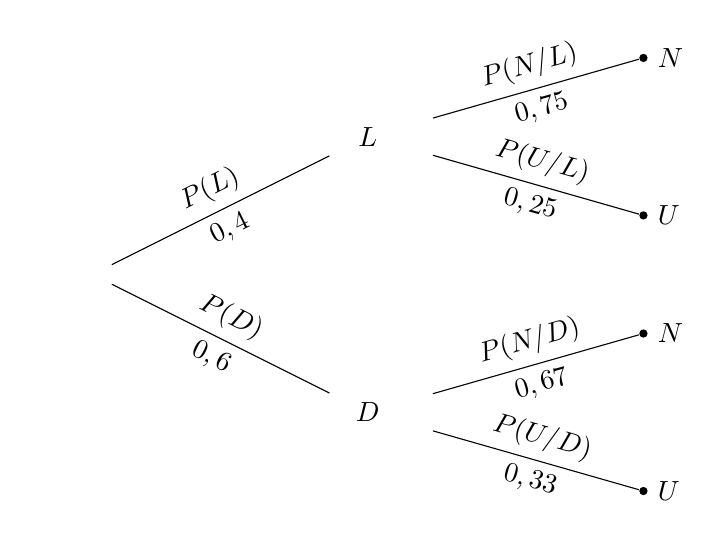
\begin{tikzpicture}[grow=right, sloped]
  %Create a start Node and childs
  \node[bag] {$  $}
  child {
    node[bag] {$D$}
        child {
                    node[end, label=right:
                        {$ U $}] {}
                    edge from parent
                    node[above] {$ P(U/D) $}
                    node[below]  {$ 0,33 $}
                }
                    child {
                                node[end, label=right:
                                    {$ N $}] {}
                                edge from parent
                                node[above] {$ P(N/D) $}
                                node[below]  {$ 0,67 $}
                            }
    edge from parent
    node[above] {$ P(D) $}
    node[below]  {$ 0,6 $}
  }
  child {
    node[bag] {$L$}
        child {
                    node[end, label=right:
                        {$ U $}] {}
                    edge from parent
                    node[above] {$ P(U/L) $}
                    node[below]  {$ 0,25 $}
                }
                    child {
                                node[end, label=right:
                                {$ N $}] {}
                                edge from parent
                                node[above] {$ P(N/L) $}
                                node[below]  {$ 0,75 $}
                            }
    edge from parent
    node[above] {$ P(L) $}
    node[below]  {$ 0,4 $}
  }
  ;
\end{tikzpicture}

        \caption{Arvore de probabilidade Desktop/Laptop/Usado/Novo }
        \label{fig:18}
      \end{figure}
      \begin{align*}
        P(D \cap U)= P(D/U)P(U)
      \end{align*}

      Ou:
      \begin{align*}
        P(D \cap U)= P(U/D)P(D)= \frac{20}{60}\times \frac{60}{100}= 0,2
      \end{align*}

    \item [Algumas propriedades]:
      \begin{enumerate}[label=(\alph*)]
        \item $P(\emptyset / B)=0$
        \item Se $A \subset \Omega$, entao $P(A^c / B)= 1-P(A/B)$
        \item Se $A,C \subset \Omega$, então:
          \begin{align}
            P(A \cup C / B)= P(A/B)+ P(C/B) - P(A \cap C/B)
          \end{align}
      \end{enumerate}

  \end{description}
  %End primeira entrega
  \section{Independência de Eventos}

  \begin{description}
    \item [Definição]: Dois eventos $A$ e $B$ definidos em $\Omega$ são independentes se 
      a informação da ocorrência ou não de $B$ não altera a probabilidade de ocorrência
      de $A$. Isto é:
      \begin{align}
        P(A/B)= P(A), \quad        P(B)>0.
      \end{align}
      Logo, dois eventos $A$ e $B$ são independentes se, e somente se, $P(A \cap B)=P(A)\times P(B)$.
    \item [Observação]: 
      \begin{align*}
        P(A/B) = \frac{P(A \cap B)}{P(B)} = \frac{P(A)P(B)}{P(B)}= P(A)
      \end{align*}
    \item [Exemplo]: Um estudante se inscreve em dois processos seletivos com probabilidade 
      $30\%$ de ser aprovado na empresa $I$ e $50\%$ de ser aprovado na empresa $II$. Se 
      as aprovações são independentes, qual a probabilidade de que ele seja aprovado em
      pelo menos uma?

      Definindo os eventos:

      \begin{enumerate}[label=\Alph*:]
        \item  O estudante ser aprovado na empresa $I$.
        \item  O esutdante ser aprovado na empresa $II$.
      \end{enumerate}
      \begin{align*}
        P(A)= 0.30\\
        P(B)=0.50\\
        P(A\cup B)= P(A)+P(B)-P(A\cap B)\\
        =P(A)+P(B)-P(A)\times P(B)\\
        =0.3+0.5- 0,3 \times 0,5\\
        =0.65
      \end{align*}
  \end{description}
  \subsection{Independência de três eventos}

  \begin{description}
    \item [Definição:]Os eventos A,B,C em $\Omega$ são independentes se e somente se:

      \begin{enumerate}[label=(\alph*)]
        \item $P(A \cap B) = P(A)\times P(B)$ 

        \item $P(A \cap C) = P(A)\times P(C)$

        \item $P(B \cap C)= P(B)\times P(C)$

        \item $P(A \cap B \cap C)= P(A)\times P(B) \times P(C)$
      \end{enumerate}

    \item [Resultado]: Se A,B são eventos independentes em $\Omega$, então:

      \begin{enumerate}
        \item $A$ e $B^c$ são independentes.
        \item $A^c$ e $B$ são independetes.
        \item $A^c$ e $B^c$ são independentes.
      \end{enumerate}
      \begin{figure}[H]
        \centering
        \def\firstcircle{(0,0) circle (1.5cm)}
\def\thirdcircle{(2,0) circle (1.5cm)}

\def \amostralspace{(-2,-2) rectangle (4,2)}
% Now we can draw the sets:
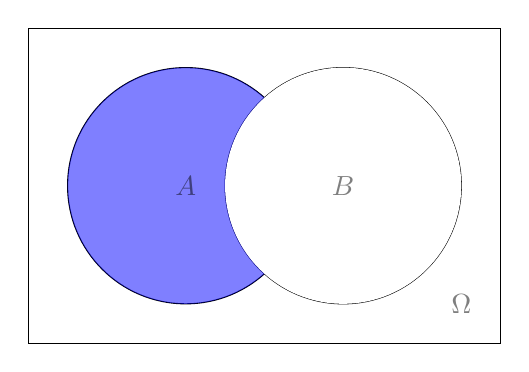
\begin{tikzpicture}
\begin{scope}[shift={(3cm,-5cm)}, fill opacity=0.5]
\draw \amostralspace ;
\node at (3.5,-1.5) {$\Omega$};
\draw \firstcircle;
\draw \thirdcircle;
\fill[blue] \firstcircle;
\fill[white,opacity=1] \thirdcircle;
\node at (0,0){$A$};
\node at (2,0) {$B$};
\end{scope}
\end{tikzpicture}

        \label{fig:19}
      \end{figure}
    \item[Prova:] Resultado $1$
      \begin{align*}
        P(A \cap B^{c})= P(A) - P(A \cap B)\\
        = P(A)-P(A)\times P(B)\\
        = P(A)(1-P(B))\\
        =P(A)\times P(B^{c})
      \end{align*}

    \item [Observação]: Não confundir eventos mutuamente exclusivos com eventos independentes. Ou seja, não confunda $P(A \cap B)  = 0$ com $ P(A \cap B) = P(A)\times P(B)$.

    \item[Exemplo]: Um atirador acerta 80\% dos disparos e outro acerta, nas mesmas condições
      acerta 70\%. Qual a probabilidade de o alvo ser acertado se ambos os atiradores disparam simultaneamente?
      \begin{enumerate}[label=\Alph*:]
        \item  Atirador 1 acerta o alvo
        \item Atirador 2 acerta o alvo
      \end{enumerate}
    \item [Resolução]:
      A intersecção de dois eventos independentes é dada pela multiplicação de suas probabilidades:
      \begin{align*}
        P(A \cap B)= P(A)P(B)\\
        =0.8 \times 0.7= 0.56
      \end{align*}
      Logo a probabilidade de interesse é dada pela a união de dois eventos:
      \begin{align*}
        P(A \cup B)= P(A)+ P(B)- P( A \cap B )\\
        = P(A) + P(B- P(A)\times P(B)\\
        = 0.8+0.7 - 0.8\times 0.7\\
        =0.94
      \end{align*}

  \end{description}
  \section{O Teorema de Bayes}
  \subsection{Partições do espaco amostral}
\item[Definição]: Uma coleção de eventos $A_1, A_2, \ldots, A_k$ formam uma partição 
  do espaço amostral $\Omega$ se:

  \begin{enumerate}[leftmargin=*, label=\Roman*., widest=IV, align=left]
    \item $A_i \cap A_j = \emptyset, \forall i\neq j$, com $i,j =1,\ldots,k$
    \item $\cup_{i=1}^{k}A_i= \Omega$
  \end{enumerate}
  \begin{figure}[H]
    \centering
    \input{tikz/Probabilidade/partition.tikz}
    \caption{Espaco amostral com $k$ particoes}
  \end{figure}
   \end{description}
   \subsection{Lema da probabilidade total}
   \begin{description}
     \item [Definição:] Se $A_1,\ldots, A_k$ é uma partição de $\Omega$, então para qualquer evento $B$ de $\Omega$, vale:

       \begin{align}
         P(B)=P\left( \sum^k_{i=1} B(B \cap A_i ) \right)\\ \nonumber
         = \sum^k_{i=1} P(B/A_i)P(A_i).
       \end{align}

       Vejamos: 

       \begin{align}
         B=  \cup_{i=1}^k \left(A_i \cap B \right) 
       \end{align}
       \begin{align}
         P(B)=P \left(\cup_{i=1}^k \left(A_i \cap B\right)\right) \\ \nonumber
         = \sum \limits_{i=1}^k P(B/A_i)P(A_i)
       \end{align}
       % \begin{figure}[htpb]
       %   \centering
       %   \caption{$B=(A_1 \cap B) \cup (A_2 \cap)\cup \dots (A_k \cap B)$ }
       %   \label{fig:20}
       % \end{figure}
   \end{description}
   \subsection{Fórmula de Bayes}
   \begin{description}
     \item [Definição] Se $A_1,A_2,\ldots, A_k$ formam uma partição de $\Omega$ e 
       $B \subset \Omega$ com $P(B)>0$, então:

       \begin{align}
         P(A_i/ B)= \frac{P(A_i \cap B)}{P(B)}\\ \nonumber
         =\frac{P(B/A_i)P(A_i)}{\sum \limits_{j=1}^k P(B/A_j)P(A_j)}
       \end{align}

     \item [Exemplo 1]: 

       Uma montadora trabalha com dois fornecedores A e B de uma determinada peça.
       Sabe-se que 10\% e 5\% das peças provenientes dos fornecedores A e B respectivamente,
       estão fora de especificação. A montadora recebe 30\% das peças do fornecedor A e 70\%
       do fornecedor B. Se uma peça do estoque inteiro é escolhido ao acaso, calcule:

       \begin{enumerate}[label=(\alph*)]
         \item A probabilidade que ela esteja fora de especificação.
         \item Se uma peça é escolhida ao acaso está fora de especificação, qual é a 
           pŕobabilidade de que tenha sido fornecido por A?
       \end{enumerate}
       \begin{enumerate}[label=\Alph*:]
         \item  Peça é do fornecedor A.
         \item  Peça é do fornecedor B.
         \item  Peça está fora de especificação.
       \end{enumerate}
       \begin{align*}
         P(A)= 0.3\\
         P(B)=0.7\\
         P(C/A)= 0.10\\
         P(C/B)= 0.05
       \end{align*}
       % \begin{figure}[htpb]
       %   \centering
       %   \caption{Name}
       %   \label{fig:21}
       % \end{figure}
       \begin{enumerate}[label=(\alph*)]
         \item $P(C)=$?

           Usando o lema da probabilidade total:
           \begin{align*}
             P(C) = P(A \cap C ) \cup P(B)\\
             P(C) = P(A \cap C) + P( B \cap C  )\\
             =P(C/A)P(A)+P(C/B)P(B)\\
             =0,1 \times 0,3 + 0.05 \times 0.7\\
             =0.065
           \end{align*}
         \item $P(A/C)=$?

           \begin{align*}
             P(A/C)= \frac{P(A\cap C)}{P(C)}\\
             = \frac{P(C/A)P(A)}{P(C/A)P(A)+P(C/B)P(B)}\\
             =\frac{0.1 \times 0.3}{0.065}=0.4615
           \end{align*}
       \end{enumerate}

     \item [Exemplo 2:]


       Estudos reveleram que 40\% dos estudantes universitários
       já experimentaram algum tipo de droga ilícita. Uma universidade resolve aplicar 
       um teste com detector de mentira para descobrir se seus estudantes já usaram algum 
       tipo de droga ilícita. Sabemos que se o estudante já usou algum tipo de droga 
       o detector vai dar positivo com certeza. Porém, sabemos que o detector erra, ou 
       seja, apresenta um falso positivo em 5\% quando aplicado em estudantes que nunca 
       usaram drogas.\\ Se um estudante é selecionado aleatoriamente e o teste aplicado 
       nele deu positivo, qual a probabilidade de ele já ter usado algum tipo de droga?

       \begin{enumerate}[label=\Alph*:]
         \item  O estudante já usou droga.
         \item  O detector deu positivo.
       \end{enumerate}
       \begin{align*}
         P(A)= 0.4 \\
         P( B / A )=1 \\
         P(B / A^c) = 0.05\\
         P(A / B)=?
       \end{align*}
       \begin{align*}
         P(A/B)= \frac{P(A \cap B)}{P(B)} \\
         = \frac{P(B/A)P(A)}{P(B/A)\times P(A) + P(B/A^c) \times P(A^c)}\\
         = \frac{1 \times 0.4}{1 \times 0.4 + 0.05 \times 0.6}\\
         =0.93
       \end{align*}
     \item  [Exercício]: Para selecionar seus funcionários uma empresa oferece aos candidatos 
       um curso de treinamento durante uma semana. No final do curso, eles são classificados
       em uma prova; 25\% são classificados como bons $(B)$, 50\% como médios $(M)$ e os 
       25\% restantes como fracos $(F)$. A empresa pretende substituir o treinamento por um teste 
       contendo questões de conhecimentos gerais. Para isso gostaria de conhecer qual a 
       probabilidade de um indíviduo aprovado no teste ser considerado fraco $(F)$, se 
       fizesse o curso. Assim, antes do início do curso, os candidatos do curso, foram 
       submetidos ao teste e receberam o conceito aprovado $(A)$ ou reprovado $(R)$. No final 
       do curso, obtiveram-se as seguintes probabilidades condicionais: 
       \begin{align*}
         P(A/B)= 0,8\\
         P(A/M) = 0,5\\
         P(A/F)=0,2
       \end{align*}
     \item [Resposta]: 0.1
   \end{description}
   \section{Variáveis Aleatórias}
   \begin{description}
     \item [Definição]: Seja um experimento aleatório e $\Omega$ o espaço amostral associado 
       a esse experimento. Uma função $X(\omega)$ que associa cada elemento $\omega \in
       \Omega$ a um número real $x=x(\omega)$ é denominada variável aleatória (v.a.\.). 
       % Espaco amostral omega em x indo para R 
       \begin{figure}[H]
         \centering
         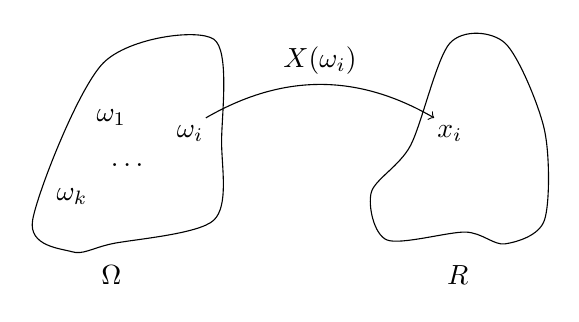
\begin{tikzpicture}
  \draw plot [smooth cycle] coordinates {(5,0.25) (6,0.35) (6.5, 0.2) (7,0.5) (7,1.65) (6.5,2.75) (5.8,2.75) (5.3,1.45) (4.8,0.85) } ;
\path[->] (2.7,1.8) edge [bend left] node[above] {$X(\omega_i)$} (5.6,1.8);
\draw plot [smooth cycle] coordinates {(1.0,.1)(1.5,.2)(2.8,.5)(2.9,1.5)(2.8,2.8)(1.4,2.5)(0.5,0.5)} ;
\node at (2.5,1.6) {$\omega_i$};
\node at (1.5, 1.8) {$\omega_1$};
\node at (1.7, 1.2) {$\dots$};
\node at (1, 0.8) {$\omega_k$};
\node at (5.8, 1.6) {$x_i$};
\node at (1.5, -0.2) {$\Omega$};
\node at (5.9, -0.2) {$\mathbb{R}$};
\end{tikzpicture}


         \caption{Representacao da variavel aleatoria que associa $\omega_i$ a um $x_i$}
         \label{fig:23}
       \end{figure}
     \item [Notação]: $X:\Omega \to \mathbb{R}$

     \item [Exemplo]: Lançamento de uma moeda duas vezes. A v.a.\ , $x$, é o $n^o$ de caras. 
       \begin{figure} [H]
         \centering
         \begin{tabular}{c c c}
           \toprule
           &c&k\\ \cmidrule{2-3}
           c&(c,c)&(c,k)\\ \cmidrule{2-3}
           k&(k,c)&(k,k)\\    \bottomrule
         \end{tabular}
         \label{tab:3}
       \end{figure}

       \begin{align*}
         \Omega : \{ \underbrace{cc}_{\omega_1};\underbrace{kc}_{\omega_2};\underbrace{kc}_{\omega_3};\underbrace{kk}_{\omega_4} \}\\
         X: \text{\quad $n^o$ de caras}\\
         X(\omega_1)= X((c,c))= x(\omega_1)=2\\
         X(\omega_2)= X((k,c))= x(\omega_2)=1\\
         X(\omega_3)= X((c,k))= x(\omega_3)=1\\
         X(\omega_4)= X((k,k))= x(\omega_4)=0\\
         R_x: \{0,1,2 \}\\
         P(x=0)=?\\
         P(x=1)=? \\
         P(x=2)=? \\
         X=
         \begin{cases}
           0, \text{\quad se ocorrer $(k,k)$} \\
           1, \text{\quad se ocorrer $(c,k)$ ou $(k,c)$} \\
           2,\text{\quad se ocorrer $(c,c)$}
         \end{cases}
       \end{align*}

     \item [Exemplo]: Em uma linha de produção, peças são classificadas em defeituosas ou não
       defeituosas. Podemos definir a v.a.\ $X$ como:
       \begin{align*}
         \begin{cases}
           x=1,\text{\quad  se a peça é defeituosa}\\ 
           0,\text{\quad  a peça não é defeituosa}
         \end{cases}
       \end{align*}
     \item [Observação]: Uma v.a.\ $X$ desse tipo é chamada de v.a.\ de Bernoulli. Nesse caso, $\Omega=\{ \text{peça defeituosa, peça não defeituosa} \}$
       % e $x$ assume um cojjunto de valores finitos.
   \end{description}
   \subsection{Classificação de Variáveis Aleatórias}
   \begin{description}
     \item [Definição :] Se a v.a.\ $X$ assume valores em um conjunto finito ou infinito e numerável é chamado 
       de variável aleatória discreta. Se $X$ assume valores, em um conjunto infinito não-enumerável,
       é chamada de v.a.\ contínua.

     \item [Exemplos]:

       \begin{enumerate}[label=(\alph*)]
         \item $x$ indica o $n^o$ de residentes em um domicílio. X pode assumir valores em $\mathbb{N}$ e assim é chamada de 
           v.a.\ discreta.

         \item $Y$ indica o tempo de vida (em horas) de um equipamento eletrônico. $Y$ pode 
           assumir valores em $\mathbb{R}^+$ e assim é chamado de v.a.\ contínua.
       \end{enumerate}
   \end{description}
   \subsection{Função Massa de Probabilidade} 
   \begin{description}
     \item [Definição]: Seja X uma v.a.\ discreta que assume valores em $R_{x}=\{x_1,x_2,\dots,
       x_{k},\dots\}$. A cada possível $x_{i}$, associamos um número, 
       \begin{align*}
         P_{i}=p({x_i})=P(X={x_i})=P(X( \omega_i)=x_i),\\
         \omega_{i} \in \Omega \quad , x_{i} \in R_{x} \nonumber
       \end{align*}
       dito probabilidade de $x_{i}$. A função $p(x)$ é definida como função massa de probabilidade 
       (f.m.p\ ) de $X$. 

       As probabilidades $p(x_i)$ devem satisfazer as seguintes condições: 
       \begin{enumerate}[label=(\roman*)]
         \item $p(x_i)>0, \forall x_i \in R_{x}$

         \item $\sum^\infty_{i=1} p(x_i)=1$
       \end{enumerate}
     \item [Interpretação da f.m.p\ ]: 

       Seja $x$ uma v.a.\ discreta com $R_{x}= \{x_1,x_2,\dots,x_k \}$ e $p(x_i)=p_i$.
       \begin{figure}[H]
         \centering
         \begin{tikzpicture}
  \begin{axis}[clip=false,
axis y line*=left,
yticklabels={$p_{2}$,$p_{n}$,$\empty$,$p_{1}$,$\empty$,$p_{k}$},ytick={1,...,6},
axis x line*=bottom,
xticklabels={$x_1$,$x_2$,$\ldots$,$x_k$,$\ldots$,$x_n$},xtick={1,...,6},xtick style={draw=none},ytick style={draw=none}
    ]
\addplot+[ycomb] plot coordinates {(1,4) (2,1) (4,6) (6,2) };
\end{axis}
\end{tikzpicture}

         \caption{Exemplo de uma função massa probabilidade}
         \label{fig:24}
       \end{figure}

     \item [Exemplo:] Lançamento de uma moeda duas vezes e $x$ é o número de caras.
       \begin{align*}
         \Omega = \{ \underbrace{cc}_{2}; \underbrace{ck}_{1};\underbrace{kc}_{1};\underbrace{kk}_{0} \} \\
         R_{x}= \{0,1,2\}
       \end{align*}
       A f.m.p de $x$ é dada por: 
       \begin{figure} [H]
         \centering
         \begin{tabular}{ c c c c}
           \toprule
           x &0&1&2 \\ \cmidrule{1-4}
           $P(x)=P(X=x)$&$1/4$&$1/2$& $1/4$\\    \bottomrule
         \end{tabular}
         \label{tab:4}
       \end{figure}


       \begin{align*}
         p(0)=P(X=0)=P((k,k))=\frac{1}{4} \\
         p(1)=P(X=1)=P((c,k))+P((k,c))=\frac{2}{4}=\frac{1}{2}\\
         p(2)=P(X=2)=P((c,c))=\frac{1}{4}\\
         P(X=x)= \begin{cases}
           \sfrac{1}{4}, \text{\quad se sair $kk$ ou $cc$ ou $x=0$ ou $x=2$}\\
           \sfrac{1}{2}, \text{\quad se sair $ck$ ou $kk$ ou $x=1$ }
         \end{cases}
       \end{align*}
       % %tabular here

     \item [Exemplo:] Um carregamento de 8 computadores contém 3 defeituosos. Se uma empresa de uma compra aleatória de dois computadores, apresente a f.m.p\ para o número de computadores com defeitos adquiridos.

       \begin{align*}   X: \text{número de computadores defeituosos}\\
         R_x = \{0,1,2\} \\
         P(X=0) = \frac{ \tbinom{3}{0} \tbinom{5}{2} }{ \binom{8}{2} }= \sfrac{5}{14}
       \end{align*}
       \begin{description}
         \item [Obs:]
           \begin{align*}
             \binom{8}{2} = \frac{8!}{2!\left( 8-2 \right)!}
           \end{align*} 
       \end{description}

       \begin{align*}
         P(X=1) = \frac{ \binom{3}{1} \binom{5}{1} }{ \binom{8}{2}}= \sfrac{15}{28} \\
         P(X=2) = \frac{ \binom{3}{2} \binom{5}{0} }{ \binom{8}{2}}=\sfrac{ 3}{28} 
       \end{align*}
       Então a f.m.p.\ é:
       \begin{figure}[H]
         \centering
         \begin{tabular}{ c c c c c}
           \toprule
           x &0&1&2&Total \\ \cmidrule{2-4}
           $P(x)$&$\frac{10}{28}$&$\frac{15}{28}$&$ \frac{3}{28}$&1\\    \bottomrule
         \end{tabular}
       \end{figure}

       %Curiosidade
     \item [Exemplo:] A demanda diária de um item é uma v.a.\ discreta com f.m.p.\ dada por: 
       \begin{align}
         P(D=d)=\frac{2^d k}{d!},\quad d=1,2,3,4
       \end{align}
       \begin{enumerate}[label=(\alph*)]
         \item Determine a constante $k$
         \item Calcule $P(D>2)$
       \end{enumerate}
       \begin{enumerate}[label=(\alph*)]
         \item Sabemos que: 
           \begin{align*}
             \sum \limits^{n}_{i=1} p(x_i)=1, \forall x_i \in R_{x}\\
             P(D=1)+P(D=2)+P(D=3)+P(D=4)=1\\
             \frac{2^1 k}{1!}+\frac{2^2 k}{2!}+\frac{2^3 k}{3!}+\frac{2^4 k}{4!}=1\\
             2K + 2K+ \frac{4K}{3}+\frac{2K}{3}=1 \\
             4K+\frac{6K}{3}=1 \\
             6K=1\\
             K=\frac{1}{6}
           \end{align*}
           Então o f.m.p de x é: 
           \begin{align*}
             P(D=d)=\frac{2^d}{6d!},\quad d=1,2,3,4
           \end{align*}
         \item 
           \begin{align*}
             P(D>2)=P(D \geq 3) \\
             =P(D=3)+P(D=4)\\
             =\frac{2^3}{6\times 3!}+ \frac{2^4}{6\times 4!}\\
             =\frac{1}{3}
           \end{align*}
           ou 
           \begin{align*}
             P(D>2)=1-P(D\le 2)\\
             = 1- \{ P(D=1)+ P(D=2) \}\\
             = 1- P(D=1)- P(D=2)
           \end{align*}
           Obs: $R_{x}: \{0,1,2,3,4,5 \}$
           \begin{align*}
             P(X>1)=P(x=2)+ P(x=3)+\cdots+P(x=5)
           \end{align*}
           ou
           \begin{align*}
             P(x>1)= 1-P(x\le 1)\\
             = 1- \{ P(x=0)+ P(x=1) \}\\
             = P(x>1)+ P(x\le 1)=1
           \end{align*}
       \end{enumerate}
   \end{description}
   \subsection{Densidade de Probabilidade}
   \begin{description}
     \item [Definição:] Seja X uma v.a.\ contínua que assume valores em $R_{x},R_{x} \in \mathbb{R}$.
       A função $f(x)$ é a função densidade de probabilidade (f.d.p) para x, se satisfaz as 
       seguintes propriedades: 

       \begin{enumerate}[label=(\roman*)]
         \item $f(x)\geq 0, \forall x \in R_{x}$
         \item $\int \limits_{R_{x}} f(x) dx=\int \limits_{-\infty}^{\infty} f(x)dx=1 $
         \item $P(a<x<b)=\int \limits^b_a f(x) dx $
       \end{enumerate}
       Uma ilustração de f.d.p: 
       %figure here
       \begin{figure}[htpb]
         \centering
         \pgfmathdeclarefunction{dnorm}{2}{%
  \pgfmathparse{1/(#2*sqrt(2*pi))*exp(-((x-#1)^2)/(2*#2^2))}%
}
\pgfmathdeclarefunction{weird}{1}{%
  \pgfmathparse{-1(-3*x^4- 35*x^2+3*x+12+100*cos(300*x )+139*sin(238*x)-120*cos(149*x)-194*sin(489*x)+9000) }%
}

\begin{tikzpicture}

\def\startx{-7}
\def\endx{7}
\def\verticalbar{6}
\begin{axis}[no markers, samples=100,
axis lines*=left, xlabel=Variavel aleatoria Continua, ylabel=f.d.p,,
height=6cm, width=10cm,  xticklabels={A,\empty,\empty,\empty,a,\empty,\empty,\empty,b,\empty,\empty,\empty,\empty,\empty,B},
xtick={-7,-6,-5,-4,-3, -2, -1, 0, 1, 2, 3,4,5,6,7}, ytick=\empty,xtick style={draw=none},
enlargelimits=false, clip=false, axis on top,
    domain=\startx:\endx
]
\addplot [name path=g5,thin, smooth] {weird(1)};
\addplot [
    fill=green!52,
    draw=none,
    domain=-3:1,
    stack plots=y
    ] {max(weird(1),0)} \closedcycle;
\node[above] at (600,300) {$P(a<x<b)$};
\end{axis}
\end{tikzpicture}

         \caption{}
         \label{fig:25}

       \end{figure}
     \item [Obs:] Se $X$ é uma v.a.\ contínua assumindo valores em $R_{x}$, então para toda 
       $a \in R_{x}$, temos: 

       \begin{enumerate}[label=(\alph*)]

         \item $P(x=a)=0$
         \item $P(x>a)=P(x\geq a)$
         \item $P(x<a)=P(x\leq a)$
         \item $P(x>a)=1- P(x \leq a)\\ = 1-P(x<a)$
         \item $P(x<a)=1-P(x \geq a)\\ 1-P(x>a)$

       \end{enumerate}

       \begin{description}
         \item Outros exemplos: 
           \begin{align*}
             P(a\le x \le b)= P(a\le x < b)\\
             = P(a<x \le b)= P(a<x<b)
           \end{align*}
         \item Obs: Só vale para v.a.\ contínua. 

       \end{description}
     \item [Exemplo:] 
       O tempo de produção de um componente (em minutos) é uma v.a.\ com função densidade 
       de probabilidade dada por: 
       \begin{align}
         f(x)=
         \begin{cases}
           \frac{5-x}{4}, \text{\quad se $2<x<4$}\\
           0,\text{\quad caso contrário} 
         \end{cases}
       \end{align}
       \begin{enumerate}[label=(\alph*)]
         \item Mostre que $f(x)$ é uma f.d.p
         \item Calcule a probabilidade de que o tempo de produção de um componente 
           seja menor do que 3 minutos.
       \end{enumerate}
       \begin{enumerate}[label=(\alph*)]
         \item Devemos verificar: 
           \begin{enumerate}[leftmargin=*, label=\roman*., widest=IV, align=left] %com os i)
             \item $f(x)\geq 0, \forall x \in R_{x}$
             \item $\int_{R_{x}} f(x)dx=1$
           \end{enumerate}

           Verificando:
           \begin{enumerate}[leftmargin=*, label=\roman*., widest=IV, align=left] %com os i)
             \item $f(x)\geq 0, \forall x \in  2<x<4$
             \item 
               \begin{align*}
                 \int_{2}^4 \frac{5-x}{4}dx=1\\
                 \int_{2}^4 5 dx - \int_{2}^4 x dx  \\
                 = \frac{1}{4}  \left(\eval{5x}{4}{2} - \eval{\frac{x^2}{2}}{4}{2}\right) \\
                 = \frac{1}{4} \left(5(4-2)- \frac{1}{2}(16-4) \right)= 1
               \end{align*}

           \end{enumerate}
           Portanto, $f(x)$ é uma função densidade de probabilidade 
         \item 
           \begin{align*}
             P(X<3)= \int \limits_{-\infty}^{(3)} f(x)dx \\
             \int \limits_{-\infty}^{2}0 dx +      \int \limits_{2}^{3} \frac{5-x}{4} dx 
           \end{align*}
           \begin{align*}
             P(X<3)=\int \limits_{2}^{3} \frac{5-x}{4} dx \\
             =            \frac{1}{4} \left(\int \limits_{2}^{3} 5 dx - \int \limits_{2}^{3} x dx \right)\\
             =\frac{1}{4} \left(5\times 1- \frac{1}{2}\times 5\right)= \frac{5}{8}\\
             P(A/B)=\frac{P(A\cap B)}{P(B)}
           \end{align*}
       \end{enumerate}
     \item [Exemplo:] Seja x uma v.a.\ contínua com f.d.p dada por:
       \begin{align*}
         f(x)= 
         \begin{cases}
           2x,\quad 0\leq x \leq 1 \\ 
           0, \quad \text{Caso contrário}
         \end{cases}
       \end{align*}
       \begin{enumerate}[label=(\alph*)]
         \item Verifique se $f(x)$ é uma f.d.p
         \item$ P \left( x\le \frac{1}{2}\right)$
         \item $P \left(X\le \frac{1}{2} / \frac{1}{3} \le x \le \frac{2}{3}\right)$
       \end{enumerate}
       \begin{enumerate}[label=(\alph*)]
         \item 
           Devemos verificar: 
           \begin{enumerate}[leftmargin=*, label=\roman*., widest=IV, align=left] %com os i)

             \item $f(x)\geq 0, \forall x \in R_{x}$

             \item $\int_{R_{x}} f(x)dx=1$
           \end{enumerate}
           Verificando:         
           \begin{enumerate}[leftmargin=*, label=\roman*., widest=IV, align=left]
             \item 
             \begin{align*}                 f(x)\geq 0, \forall x \in  0<x<1\end{align*}
             \item 
               \begin{align*}
                 \int \limits_{R_x} 2x dx
                 =\int \limits_{0}^1 2x dx\\ 
                 = \eval{\frac{2x^2}{2}}{1}{0}= 1
               \end{align*}

           \end{enumerate}


           Portanto, $f_x(x)$ é uma f.d.p.\

         \item 
           \begin{align*}
             P(X \leq 1/2) = \int \limits_{-\infty}^{\sfrac{1}{2}} f_x (x) dx\\
             = \int \limits_{-\infty}^0 0 dx + \int \limits_{0}^{\sfrac{1}{2}} 2x dx \\
             = \eval{x^2}{{\sfrac{1}{2}}}{0}\\
             =\frac{1}{4} 
           \end{align*}
         \item Probabilidade Condicional
           \begin{figure}[H]
             \centering
             
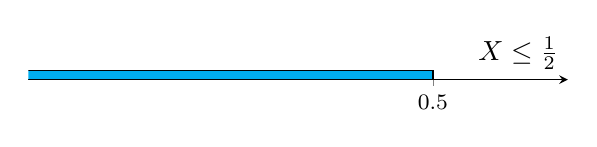
\begin{tikzpicture}
\begin{axis}[%
compat=newest, %footnotesize
tick label style={font=\footnotesize},
label style={font=\small},
legend style={font=\small},
axis x line = center,
axis y line = center,
every axis/.style={pin distance=1ex},
trim axis left,
axis x line=center,
axis y line=none,
xmin=-1,xmax=1,
ymin=0, ymax= 1,
xtick={0.5},
xlabel= $X \leq \frac{1}{2}$
]
\addplot[fill=cyan,domain=-10:0.5] {0.02}\closedcycle;
\end{axis}
\end{tikzpicture}
\hfill
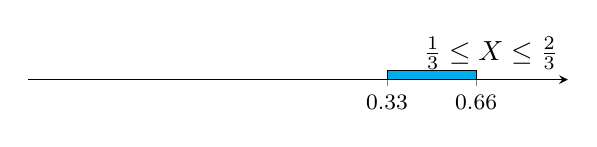
\begin{tikzpicture}
\begin{axis}[compat=newest, %footnotesize
tick label style={font=\footnotesize},
label style={font=\small},
legend style={font=\small},
axis x line = center,
axis y line = center,
every axis/.style={pin distance=1ex},
trim axis left,
axis x line=center,
axis y line=none,
xmin=-1,xmax=1,
ymin=0, ymax= 1,
xtick={0.33,0.66},
xlabel= $\frac{1}{3} \leq X \leq \frac{2}{3}$
]
\addplot[fill=cyan,domain=0.33:0.66] {0.02}\closedcycle;
\end{axis}
\end{tikzpicture}
\hfill
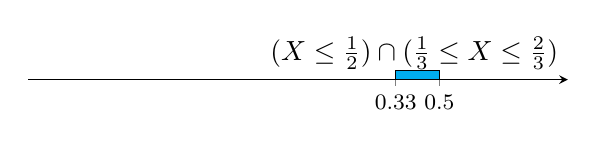
\begin{tikzpicture}
\begin{axis}[compat=newest, %footnotesize
tick label style={font=\footnotesize},
label style={font=\small},
legend style={font=\small},
axis x line = center,
axis y line = center,
every axis/.style={pin distance=1ex},
trim axis left,
axis x line=center,
axis y line=none,
xmin=-1.1,xmax=1,
ymin=0, ymax= 1,
xtick={0.33,0.5},
xlabel=  $ (X \leq \frac{1}{2} )\cap (\frac{1}{3} \leq X \leq \frac{2}{3})$
]
\addplot[fill=cyan,domain=0.33:0.5] {0.02}\closedcycle;
\end{axis}
\end{tikzpicture}

             \label{fig:26}
           \end{figure}
           \begin{align*}
             P(A/B)= \frac{P(A\cap B)}{P(B)} \\
             \frac{ P\left( X \leq \frac{1}{2} \right)\cap P \left(\frac{1}{3} \leq X \leq \frac{2}{3}\right)}{P \left( \frac{1}{3} \leq X \leq \frac{2}{3}\right)}\\
             = \frac{P( \frac{1}{3} \leq X \leq \frac{1}{2} )}{P( \frac{1}{3} \leq X \leq \frac{2}{3} )}\\
             = \frac{\int \limits_{\frac{1}{3}}^{\frac{1}{2}} 2x dx}{\int \limits_{\frac{1}{3}}^{\frac{2}{3}} 2x dx} \\
             = \frac{\eval{x^2}{{\frac{1}{2}}}{{\frac{1}{3}}}}{ \eval{x^2}{{\frac{2}{3}}}{{\frac{1}{3}}}}\\
             = \frac{5}{12}
           \end{align*}
       \end{enumerate}

   \end{description}
   \subsection{Função distribuição acumulada discreta}
   \begin{description}
     \item [Definição:] Seja x uma v.a.\ discreta que assume valores em $R_{x}$ e com f.m.p.\
       $p(x)=P(X=x)$. Para qualquer $x \in \mathbb{R}$, a função de distribuição 
       acumulada(f.d.a) de x, denotada por $F_{x}(x)$, é definida como: 
       \begin{align}
         F_{x}(x)=P(X \leq x )= \sum \limits_{x_{i} \in R_{x}} P(X=x_i) = \sum_{x_{i} \in R_{x}} p(x_i) , \quad        \forall x_i \le x \nonumber
       \end{align}
       De forma mais clara, temos como exemplo: 
       \begin{align*}
         R_{x}= \{0,1,2,3,4 \}\\
         F_{x}(2,3)= P(X\le 2,3)\\
         = P(x=0)+P(x=1)+P(x=2)
       \end{align*}
     \item [Exemplo:]
       Conidere o lançamento de uma moeda duas vezes e x é o número de caras. Já sabemos
       que a f.m.p de x é dada por:
       \begin{figure} [H]
         \centering
         \begin{tabular}{c c c c}
           \toprule
           x&0&1&2\\ \midrule
           $P(X=x)$&$\frac{1}{5}$&$\frac{1}{2}$&$\frac{1}{4}$\\ \bottomrule
         \end{tabular}
         \label{tab:5}
         %\caption{F.m.p do lançamento de uma moeda}
       \end{figure}
       Com $R_{x}=\{0,1,2\}$\\
       Ou, de forma equivalente podemos escrever: 
       \begin{align*}
         p(x)=P(X=x)=
         \begin{cases}
           \frac{1}{4}, \quad \text{se} \quad x=0,2\\
           \frac{1}{2}, \quad \text{se} \quad x=1\\
           0,\quad  \text{caso contrário}
         \end{cases}
       \end{align*}
       A f.d.a de x é dada por:
       \begin{align*}
         F_{x}=P(X\le x)= 
         \begin{cases}
           0,\quad  x<0 \\
           \frac{1}{4}, \quad 0 \le x <1\\
           \frac{3}{4}, \quad 1 \le x < 2\\
           1, \quad x \geq 2
         \end{cases}
       \end{align*}

       A representação gráfica de $F_x(x)$ é: 
       \begin{figure}[H]
         \centering
         \def\startx{-2}
\def\endx{4}
\begin{tikzpicture}
\begin{axis}[
axis lines*=left,enlargelimits=false, clip=false, axis on top,
domain=\startx:\endx]S
\addplot[color=blue,thick,domain=-3:0,ultra thick]{0};
  \addplot+[no markers,color=blue,domain=0:1,ultra thick]{0.25};
  \addplot+[no markers,color=blue,domain=1:2,ultra thick]{0.75};
  \addplot+[no markers,color=blue,domain=2:5,ultra thick]{1};
  \addplot[mark=*,solid,color=blue,fill=blue] coordinates {(1,0.75)};
  \addplot[mark=*,solid,color=blue,fill=blue] coordinates {(0,0.25)};
  \addplot[mark=*,solid,color=blue,fill=blue] coordinates {(2,1)};
  \addplot[mark=*,solid,color=blue,fill=white] coordinates {(2,0.75)};
  \addplot[mark=*,solid,color=blue,fill=white] coordinates {(1,0.25)};
\end{axis}
\end{tikzpicture}

         \caption{}
         \label{fig:}
       \end{figure}
       % % grafico aqui
   \end{description}
   \subsection{Função distribuição acumulada contínua}
   \begin{description}
     \item [Definição:] Seja x uma v.a.\ contínua que assume valores em $R_{x}$ e com 
       f.d.p $f(x)$. Para qualquer $x \in \mathbb{R}$, a f.d.p de $x$, denotada por 
       $F_{x}(x)$ é definida como: 
       \begin{align}
         F_{x}(x)= P(X \leq x)= \int \limits_{-\infty}^{x} f(t)dt 
       \end{align}
     \item [Observação:] $F_{x}(x)= P(X \leq a)= \int \limits_{-\infty}^{a}f(t)dt  , \quad a \in \mathbb{R}$

       Como consequência imediata podemos escrever dois resultados: 
       \begin{align}
         P(a <x<b)= \int \limits_{a}^{b} f(x)dx\\
         = F_{x}(b)-F_{x}(a)
       \end{align}
       %fig here showing a and b interval
       % E: 

       \begin{align}
         f(x)=\frac{\partial F_{x}(x)}{\partial x}, \text{\quad se a derivada existir}
       \end{align}

     \item [ Exemplo: ] Considere a f.d.p dada por: 
       \begin{align*}
         f(x)= 
         \begin{cases}
           \frac{x^2}{3},\quad  -1 < x < 2 \\
           0, \quad \text{caso contrário}
         \end{cases}
       \end{align*}
       Determine $F_{x}(x)$ e use-a para avaliar $P(0 \le x< 1)$.

       A f.d.a de x é dada por: 
       \begin{align*}
         F_{x}(x)= P(X \le x)= \int \limits_{-\infty}^{x} f_{x}(t) dt\\
         = \int \limits_{-\infty}^{x} \frac{t^2}{3} dt , \quad -1<t<2 \\
         \int \limits_{-1}^{x} \frac{t^2}{3} dt= \frac{1}{9} \eval{t^3}{-1}{x}\\
         F_{x}(x)= \frac{1}{9}\left(x^3 +1\right)\\
       \end{align*}
       \begin{align*}
         F_{x}(x)=P(X \le x)= 
         \begin{cases}
           0, x <-1 \\
           \frac{1}{9}(x^3 +1) , -1 \le x <2 \\
           1, x \geq 2
         \end{cases}
       \end{align*}
       \begin{align*}
         P(0 \le x <1)=? \\
         P(0 \le x <1)= {F}_{x}(1)- {F}_{x}(0)\\
         P(x \le 1 ) - P(x \le 0)= \frac{1}{9} (1^3 + 1 ) - \frac{1}{9}(0^3+ 1)\\
         P(0 \le x < 1 )= \frac{2}{9} - \frac{1}{9} = \frac{1}{9}
       \end{align*}
       Ou 
       \begin{align*}
         P(0 \leq X < 1) = \int \limits_{0}^{1} \frac{x^2 }{3}dx 
       \end{align*}
       % %fig de uma reta de -1 a 2 num plano 
       % O comportamento gráfico de $\mathbb{F_{x}}(x)$ é: 
       % % grafico da função aqui $
   \end{description}
   \subsection{Propriedades de f.d.a}
   \begin{enumerate}[label=(\alph*)]
     \item ${F}_{x}(x)$  é uma função contínua.
     \item ${F}_{x}(x)$ é uma função monótona não decrescente. 
     \item  $0 \le {F}_{x}(x)\le 1,\quad \forall x \in \mathbb{R}$
     \item $ \lim \limits_{x \to -\infty} {F}_{x}(x)=0$ e $ \lim \limits_{x \to +\infty} {F}_{x}(x)=1$
     \item $P(x \le a) = {F}_{x}(a)$
     \item $P(x>a)=1 - P(x \le a)= 1 - {F}_{x}(a)$
     \item $P(a<x\le b)= {F}_{x}(b)- {F}_{x}(a)$
   \end{enumerate}
   \begin{description}

     \item [Exemplo:] 
       Seja $x$ uma v.a.\ contínua com f.d.p dada por:
       \begin{align*}
         f_{x}(x) = 
         \begin{cases} 
           k x^2, 0 < x < 1 \\
           0, \quad \text{c.c.\ }
         \end{cases}
       \end{align*}
       \begin{enumerate}[label=(\alph*)]
         \item Achar $k$.
         \item Determine ${F}_{x} (x)$.
         \item $P (\frac{1}{3} < x < \frac{1}{2})$
       \end{enumerate} 

       \begin{enumerate}[label=(\alph*)]
         \item 

           \begin{align*}
             \int \limits_{R_x} f(x) dx =1 \\
             k \int \limits_{0}^{1} x^2 dx = 1 \\
             \frac{k}{3} \eval{x^3}{0}{1} = 1 \\
             \frac{k}{3}=1 \therefore k=3
           \end{align*}
           Logo, a f.d.p de $X$ é:
           \begin{align*}
             f_x(x)= \begin{cases}
               3x^2, \quad 0<x<1 \\
               0 , \quad \text{c.c.\ }
             \end{cases}
           \end{align*}
         \item  ${F}_{x} (x)= ?$
           \begin{align*}
             F_{x}= P(X \leq x)= \int \limits_{-\infty}^{x} f_{x} (t) dt \\
             = \int \limits^{x}_{0} 3 t^2 dt
             = \eval{t^3}{{x}}{{0}}= x^3
           \end{align*}
           Assim, a f.d.a.\ é dada por:
           \begin{align*}
             F_x(x)= \begin{cases}
               0 , \quad  x<0\\
               x^3, \quad 0 \leq x<1 \\
               1 , \quad x \geq 1 
             \end{cases}
           \end{align*}
         \item 
           \begin{align*}
             P\left( \frac{1}{3}< X < \frac{1}{2} \right)= F_{x} \left(\frac{1}{2}\right) - F_{x} \left(\frac{1}{3}\right)\\
             = \left(\frac{1}{2}\right)^3 - \left(\frac{1}{3}\right)^3 \\
             = \frac{1}{8} - \frac{1}{27}\\
             = \frac{19}{216}
           \end{align*}
           Ou 
           \begin{align*}
             P \left( \frac{1}{3} < x < \frac{1}{2} \right)= \int \limits_{\frac{1}{3}}^{\frac{1}{2}} 3x^2 dx = \frac{19}{216}
             \end{align*}
         \end{enumerate}
         % Obs: Se x é uma v.a.\ contínua, então $P(x=a)=0, \forall a$ com isso vale: 
         % \begin{align}
         %   P(x<a)=\mathbb{F_{x}}(a)\\
         %   P(a<x<b)= P(a \le x < b)= P(a < x \le b)\\
         %   = P(a \le x \le b)=\mathbb{F_{x}}(b)-\mathbb{F_{x}}(a)
         % \end{align}
       \item  [Exemplo:]
       \item  Seja $F_{x}$ dada por:
         \begin{align*}
           F_{x}=\begin{cases} 
             0, \text{\quad se }x<0 \\
             \frac{1}{8},\text{\quad se }0 \le x <1 \\
             \frac{1}{2}, \text{\quad se }1 \le x < 2 \\
             \frac{5}{8}, \text{\quad se }2 \le x < 3 \\
             1,\quad \text{se } x \geq 3
           \end{cases}
         \end{align*}

         Determine: 
         \begin{enumerate}[label=(\alph*)]
           \item $P(1 < x \le 3)$
           \item $P(x>2)$
           \item Encontre a $P(x)$
         \end{enumerate}
         \begin{enumerate}[label= (\alph*)]
           \item 
             \begin{align*}
               P(1 \le X \le 3)= F_{x}(3) - F_{x}(1) = \frac{1}{2}
             \end{align*}
           \item 
             \begin{align*}
               P( X > 2)=1 - F_{x}(2) \\
               = 1- F_{x}(2)= 1 - \frac{5}{8}= \frac{3}{8}
             \end{align*}

           \item
             \begin{align*}
               F_{x}(0)= P(X \le 0)= \frac{1}{8}\\
               P(X=0)= \frac{1}{8}
             \end{align*}
             \begin{align*}
               F_{x}(1)= P(X \le 1)= \frac{1}{2}\\
               P(X=0)+P(X=1)= \frac{1}{2} \\
               P(X=1)= \frac{1}{2}- \frac{1}{8}= \frac{3}{8}
             \end{align*}
             \begin{align*}
               F_{x}(2)= P(X \le 1)= \frac{5}{8}\\
               P(X=0)+P(X=1)+P(X=2)= \frac{5}{8}\\
               F_{x} (1) + P(X \le 2 )=\frac{5}{8}\\
               P(X=2)= \frac{5}{8}- \frac{1}{2}= \frac{1}{8}
             \end{align*}
             \begin{align*}
               F_{x}(3)= P(X \le 3)= 1\\
               \underbrace{P(X=0)+ P(X=1)+ P(X=2)}_{F_{x}(2)} + P(X=3)=1\\
               P(X =3) = 1- \frac{5}{8}= \frac{3}{8}
             \end{align*}

Assim temos:
             \begin{figure}[H]
               \centering
         \begin{tabular}{c c c c c}
           \toprule
           x&0&1&2&3\\ \cmidrule{2-5}
           $P(X=x)$&$\frac{1}{8}$&$\frac{3}{8}$&$\frac{1}{8}$&$\frac{3}{8}$\\ \bottomrule
         \end{tabular}
         \label{tab:6}
       \end{figure}
         \end{enumerate}
       \end{description}
     \section{Esperança Matemática de uma Variável Aleatória}
     \begin{description}
       \item [Definição:] Seja $X$ uma v.a.\ com f.m.p.\ $p_{x}(x)$ (no caso discreto) ou f.d.p
         $f_{x}(x)$ (no caso contínuo). Chamamos de esperança matemática ou valor médio 
         de $X$ ao valor: 
         \begin{align}
           \mu_{x}= E(X)= \sum \limits_{x \in R_{x}} x p_{x)}(x) , 
           \text{\quad no caso discreto}\\
           \mu_{x}= E(X)= \int_{x \in R_{x}} x f_{x}(x)dx, \text{\quad no caso contínuo}
         \end{align}

         Considerando $a,b \in \mathbb{R}$, constantes, temos  algumas propriedades:

         \begin{enumerate}[label=(\alph*)]
           \item 
             \begin{align}
               E(aX)=aE(x)
             \end{align}
           \item Se $X=a$, 
             \begin{align}
               E(X)=E(a)=a
             \end{align}
           \item 
           \begin{align}    E(E(X))= E(X)\end{align}
           \item 
           \begin{align}  E(pm a)=E(X)\pm a\end{align}
\item 
\begin{align}  E(ax + b)=aE(X)+ b\end{align}

           \item 
           \begin{align}  E(ax + by)=aE(X)+ b E(Y)\end{align}
         \end{enumerate}
       \item [Exemplo:]Considere a v.a.\ $x$ com f.d.p dada por: 
         \begin{align*}
           f_{x}(x)=\begin{cases}
             2x,\quad 0\le x \le 1 \\
             0, \text{\quad caso contrário}
           \end{cases}
         \end{align*}
         Calcular o $E(X)$:
         \begin{align*}
           E(X)=\int_{R_{x}} x f_{x}(x)dx
         \end{align*}
         \begin{align*}
           E(X)=\int \limits_{0}^{1} x\times 2xdx=2 \int \limits_{0}^{1} x^{2}dx \\
           = \frac{2}{3} \eval{x^{3}}{0}{1} = \frac{2}{3}
         \end{align*}

         % Exemplo: Seja $X$ uma v.a.\ com f.m.p.\ dada por:
         % \begin{align}p_{x}(x)=\frac{\binom{4}{x}\binom{3}{3-x}}{\binom{7}{3}}, x=0,1,2,3\end{align}
         % Calcule o $E(X)$.

         % \begin{align}
         %   (X)=\sum \limits_{(x \in R_{x})} x P(X=x)\\
         %   p_{x=0}(x)=\frac{\binom{4}{0}\binom{3}{3-0}}{\binom{7}{3}}=\frac{1}{35}\\
         %   p_{x=1}(x)=\frac{\binom{4}{1}\binom{3}{3-1}}{\binom{7}{3}}=\frac{12}{35}\\
         %   p_{x=2}(x)=\frac{\binom{4}{2}\binom{3}{3-2}}{\binom{7}{3}}=\frac{18}{35}\\
         %   p_{x=3}(x)=\frac{\binom{4}{3}\binom{3}{3-3}}{\binom{7}{3}}=\frac{4}{35}
         % \end{align}
         % \begin{align}
         %   E(X)=0 P(X=0)+1 P(X=1)+2 P(X=2)+3 P(X=3)\\
         %   =0 \frac{1}{35}+1 \frac{12}{35}+3 \frac{2\times 18}{35}+ 3 \frac{4}{35}\\
         %   =\frac{60}{35}=1,71
         % \end{align}

       \item [Resultado:] Seja $X$ uma v.a.\ com f.m.p $p_{x}(x)$ ou f.d.p $f_{x}(x)$. Uma função
         de $X$, dita $g(x)$, é também uma v.a.\ e: 
         \begin{align}
           \mu=E\left(g(x)\right)=\sum \limits_{x \in R_{x}} g(x)p_{x}(x)
           =\sum \limits_{x \in R_{x}} g(x)P(X=x), \text{\quad no caso discreto} \nonumber \\
        \mu=   E\left(g \left(x \right)\right)=\int \limits_{R_{x}} g(x)f_{x}(x)dx, \text{\quad no caso contínuo}
         \end{align}

     \end{description}
     % Exemplo:\\ Seja $X$ uma v.a.\ com f.m.p dada por: 
     % \begin{align}
     %   p_{x}=\begin{cases}
     %     \frac{1}{2}, \text{\quad} x=0\\
     %     \frac{1}{4}, \text{\quad}x=1,2\\
     %     \frac{1}{2}, \text{\quad 0 caso contrário}
     %   \end{cases}
     % \end{align}
     % Considere a v.a.\ $g(x)={(x-a)}^2$, $a=0,\frac{1}{2},1$. Calcule: 
     % \begin{enumerate}[label=(\alph*)]
     %   \item $E(x)$
     %   \item $E(g(x))$ para cada $a$.
     % \end{enumerate}

     % \begin{enumerate}[label=(\alph*)]
     %   \item 
     %     \begin{align}
     %       E(X)=0 \times \frac{1}{2}+ 1 \times \frac{1}{4}+ 2 \times \frac{2}{4}\\
     %       =\frac{3}{4}
     %     \end{align}
     %   \item 
     %     \begin{align}
     %       E(g(x))=E({(x-a)}^2)\\
     %       =\sum \limits_{(x \in R_{x})}(x-a)^2P(X=x)
     %     \end{align}
     %     ou
     %     \begin{align}
     %       E(g(x))=E(x^2-2ax+a^2)\\
     %       =E(x^2)-2aE(x)+a^2
     %     \end{align}
     %     \begin{align}
     %       E(x^2)=\sum \limits_{(x \in R_{x})} x^2 P(X=x)\\
     %       =0^2 \frac{1}{2}+1^2 \frac{1}{4}+ 2^2 \frac{1}{4}\\
     %       =\frac{5}{4}
     %     \end{align}
     %     \begin{align}
     %       E(g(x))=\frac{5}{4}-2a \frac{3}{4}+a^2\\
     %       =\frac{5}{4}-\frac{6}{4}a+a^{2}
     %     \end{align}
     %     Para $a=0$:
     %     \begin{align}
     %       E(g(0))=\frac{5}{4}-2\times 0 \frac{3}{4}+0^2\\
     %       =\frac{5}{4}-\frac{6}{4}0+0^{2}\\
     %       =\frac{5}{4}
     %     \end{align}
     %     Para $a=\frac{1}{2}$:
     %     \begin{align}
     %       E(g(\frac{1}{2}))=\frac{5}{4}-2\times \frac{1}{2} \frac{3}{4}+\frac{1}{2}^2\\
     %       =\frac{5}{4}-\frac{6}{4}\frac{1}{2}+\frac{1}{2}^{2}\\
     %       =\frac{1}{4}
     %     \end{align}
     %     Para $a=1$:
     %     \begin{align}
     %       E(g(1))=\frac{5}{4}-2\times 1 \frac{3}{4}+1^2\\
     %       =\frac{5}{4}-\frac{6}{4}1+1^{2}\\
     %       =\frac{3}{4}
     %     \end{align}
     % \end{enumerate}
     \section{Variância}

     \begin{description}
       \item [Definição:] Seja $x$ uma v.a.\ com f.m.p $p_{x}(x)$ ou f.d.p $f_{x}(x)$, com 
         média $\mu_{x}=E(x)$. Chamamos de variância da v.a.\ $X$ o valor: 
         \begin{align}
           \sigma^2=var(x)=E\left(\left(X-E\left(X\right)\right)^2\right)\\
           =E \left((x-\mu)^2\right),
         \end{align}
         Ou seja,
         \begin{align}
           \sigma^2 =var(x)=\sum \limits_{x \in R_{x}} (x-\mu_{x})^2 P(X=x) \text{\quad no caso discreto)}\\
           \sigma^2 =var(x)=\int_{R_{x}} (x-\mu_{x})^2 f_{x}(x)dx \text{\quad no caso contínuo}
         \end{align}
         A raíz quadrada da variância$(\sqrt{\sigma^2}=\sqrt{var(x)})$ é o desvio padrão, 
         denotado por $\sigma$.

       \item [Resultado:] Podemos escrever a variância v.a.\ $x$ por: 
         \begin{align}
           \sigma^2 =var(x)=E(X^2)-\left(E(X)\right)^2\\
           \sigma^2 =E(X^2)-\left(\mu_x\right)^2
         \end{align}
       \item [Demonstração:] 
         \begin{align}
           var(x)=E(x^2-2\mu_{x}x+\mu_{x}^2)\\
           =E(x^2)-2\mu_{x}E(x)+\mu_{x}^2\\
           =E(x^2)-2\mu_{x}\mu_{x}+\mu_{x}^2\\
           =E(x^2)-\mu_{x}\\
           =E(x^2)-\left(E(x)\right)^2
         \end{align}
       \item [Obs:] $E(x^2) \neq \left(E(x)\right)^2$

       \item [Propriedades]

         Considerando $a,b \in \mathbb{R}$, constantes:
         \begin{enumerate}[label=(\alph*)]
           \item 
             \begin{align*}
             Var(ax)=a^2Var(x)
           \end{align*}
             \begin{description}
               \item[Obs:] $Var(-x)=Var(x)$
           \end{description}
           \item Se $x=a$, então:
             \begin{align*}
Var(x)=Var(a)=0
           \end{align*}
         \item 
           \begin{align*}
             Var(x \pm a)=Var(x)Var(a)=Var(x)
           \end{align*}
           \item Se $a,b$ são constantes,

              \begin{align*}
               Var(ax+\pm+b)=a^2 Var(x)+Var(b)\\
             =a^2 var(x)
             \end{align*}
           \item Se $x$ e $y$ são duas v.a.'s independetes, então: 
\begin{align*}
               Var(ax \pm by)=a^2 Var(x)+ b^2 Var(y)
\end{align*}
         \end{enumerate}
       \item [Exemplo:] Seja $x$ uma v.a.\ com f.d.p\ dada por: 
         \begin{align}
           f_{x}=
           \begin{cases}
             \frac{x^2}{3}, \text{\quad} -1<x<2\\
             0, \text{\quad caso contrário}
           \end{cases}
         \end{align}
         \begin{description}
           \item [Encontre]:
         \begin{enumerate}[label=(\alph*)]
           \item $E(X)$
           \item $Var(X)$
           \item $E(4X+3)$
           \item $Var(4X+3)$
         \end{enumerate}
       \item [Resolução]:
         \begin{enumerate}[label=(\alph*)]
           \item 
             \begin{align*}
               \mu= E(X)=  \int \limits_{-1}^{2}\frac{x\times x^2}{3)}dx\\
               =\frac{1}{3}\int \limits_{-1}^{2}x^3dx=\frac{1}{12} \eval{x^4}{-1}{2}\\
               =\frac{1}{12}(16-1)=\frac{15}{12}
             \end{align*}
           \item 
             \begin{align*}
               Var(x)=E(x^2)-\left(E(x)\right)^2\\
               E(x^2)=\int \limits_{-1}^{2} x^2 \frac{x^2}{3}dx
               =\frac{1}{3}\int{-1}{2} x^4 dx\\
               =\frac{1}{15}\eval{x^5}{-1}{2}
               =\frac{1}{15}(32+1)=\frac{33}{15}\\
               Var(x)=\frac{33}{15}-\left(\frac{15}{12}\right)^2=0,6375
             \end{align*}
           \item 
             \begin{align*}
               E(4x+3)=4E(x)+3
               =8
             \end{align*}
             \begin{description}
             Obs: $E(ax)= a^2 var(x)$
           \end{description} 
         \item 
           \begin{align*}
             Var(4x+3) = 16 Var(x)= \frac{51}{80}\times16= 10,2
           \end{align*}
         \end{enumerate}
       \end{description}
     \end{description}
